\documentclass[12pt]{article}

\usepackage[a4paper, margin = 1in]{geometry}
\usepackage{graphicx}

\usepackage{xcolor}
\usepackage[pdfborderstyle={/S/U/W 1}]{hyperref}

\usepackage{biblatex}
\addbibresource{references.bib}

\hypersetup{
    pdfborderstyle={/S/U/W 1},
    breaklinks=false,
    colorlinks=true,
    linkcolor=black,
    citecolor=blue,
    filecolor=magenta,      
    urlcolor=blue,
}

\urlstyle{same}

\linespread{1.15}

\title{COMP3217 COURSEWORK 2}
\author{MUHAMAD ABEED SAHARUDIN (STUDENT ID: 33371806)}
\date{\today}

\begin{document}

    \maketitle

    \section{Problem Statement}

        The problem that were given is to detect physical cyber-attacks on a power system framework configuration using 
        machine learning (ML). There are many different scenarios that can happen on the framework that can indicate
        whether a physical cyber attack is targeted towards the framework \cite{cw-readme}, however for this coursework 
        only 3 are described and analysed, which are natural faults, data and remote command injection attacks, and
        normal events.

        This coursework is divided into 2 parts. The first part is concerned with only detecting between normal events 
        and data injection attack events. The second part is concerned with the same events, with the addition of 
        remote command injection attack events.
        
        This report explains the data composition, ML pipeline design, and training evaluation for both
        parts of the courswork.

    \section{Data Composition}

        The training data given to train the ML algorithm are 2 \verb|csv| files, each containing 6,000  system traces, 
        with each of those containing 128 features. The first training file is for the first part of this coursework, 
        where the last column is a marker that serves as a label indicating whether an event to the framework is a 
        normal event (labelled as 0) or a data injection attack event (labelled as 1). The second file is for the
        second part of this coursework, which contains the same data marker, with the addition of the third event, a 
        remote command injection attack (labelled as 2).

        
        \begin{figure}[h]
            \centering
            \includegraphics[]{}
        \end{figure}

        % I CAN'T WITH FIGURES FFS
        % \begin{figure}[h]

        %     \begin{minipage}[c]{0.3\linewidth}
        %         \centering
        %         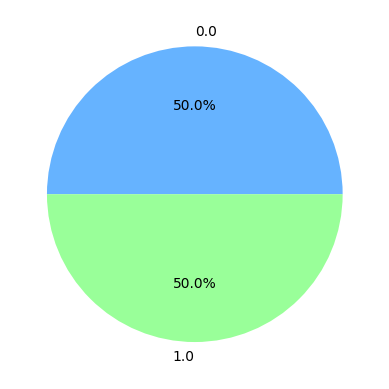
\includegraphics[width = \linewidth]{figures/binary-marker}
        %         \caption{Image A}
        %     \end{minipage}

        %     \hfill

        %     \begin{minipage}[c]{0.3\linewidth}
        %         \centering
        %         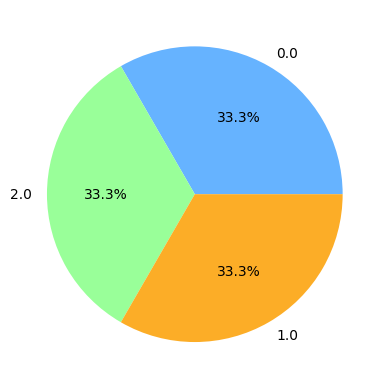
\includegraphics[width = \linewidth]{figures/multi-marker}
        %         \caption{Image B}
        %     \end{minipage}

        % \end{figure}
    
    \section{ML Pipeline Design}

    It is required that the design of the ML workflow be done in Google Notebook. The link is provided in the
    \hyperref[sec:references]{References} section \cite{binary_dataset, multi_dataset}. 

        \subsection{Pre-Processing}

            Before training, data pre-processing was done to better prepare the ML models for maximum performance on
            training and better generalisation on unseen data. One of the pre-processing methods used is standardising
            the dataset so its data distribution has mean 0 and unit variance.  

        \subsection{ML Models}

            For this coursework, the \verb|RandomForest| classifier from \verb|scikit-learn| was used to 

    \section{Training Evaluation}

    \section{Conclusion}

    \newpage

    \section{References}
    \label{sec:references}
    
        \printbibliography[heading = none]

\end{document}